\section{Spezifikation der Inventursoftware}

Die Inventursoftware besteht aus einer einfachen Client-Server Anwendung. Die Client-Anwendung zeigt das Live-Drohnenbild mit den eingezeichneten, erkannten Objekten. Zudem wird die Anzahl an erkannten Objekten der spezifischen Klassen rechts daneben dargestellt. Wann die Drohne die Inventur durchführen soll, wird auf Initiative des Benutzers gestartet. 

\begin{figure}[ht]
	\begin{center}
		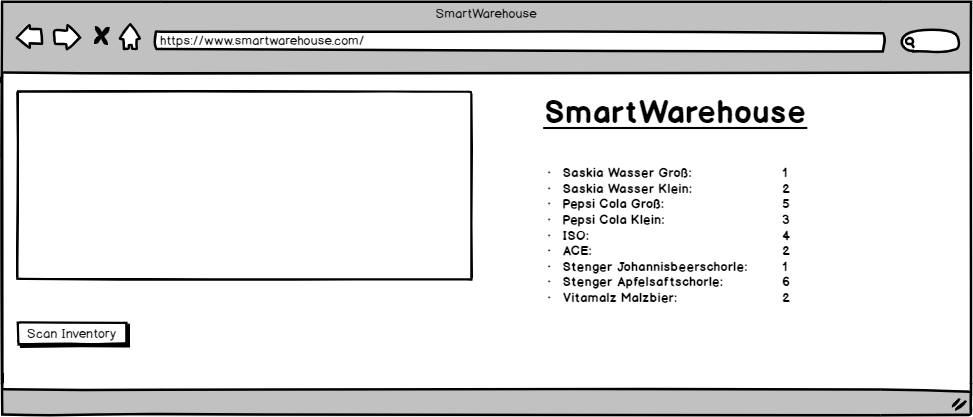
\includegraphics[width=15cm]{Bilder/UI.png} 
		\caption[SmartWarehouse User Interface]{SmartWarehouse User Interface}
		\label{ui}
	\end{center}
\end{figure}

Der Server, geschrieben im \textit{Django} Framework für Python, verbindet sich zu Drohne und weißt deren Flugsequenzen an. Auf ihm ist das \textit{Deep Learning} Modell deployt. Der Server inferiert die von der Drohne empfangenen Video-Stream-Frames mit dem Modell und gibt diese anschließend an die Client Applikation weiter. Eine \textit{REST} Schnittstelle gibt Aussage über die Bestandsdaten des Warenhauses.